\chapter{Security Challenges in Smart Constracts}
\markboth{Title of My Seminar Work}{}
\chaptauthors{Lucas Pelloni and Ile Cepilov}

\Kurzfassung{%
This is the abstract.
It fits pretty much on one page and is definitely not longer.}

\newpage

\minitoc %table of contents

\newpage
%http://blockgeeks.com/guides/what-is-blockchain-technology/
%http://www.investopedia.com/terms/b/blockchain.asp
%https://letstalkpayments.com/an-overview-of-blockchain-technology
% PWC: PAPER DA PRENDERE ASSOLUTAMENTE http://www.pwc.ch/en/2017/pdf/pwc_blockchain_opportunity_for_energy_producers_and_consumers_en.pdf


\section{Blockchain Technology}
\subsection{What is a Blockchain?}
A blockchain is like a distributed database which constantly keeps a list of transaction or records, that have ever been executed, called usually blocks. Every record contains a reference to its predecessor and a timestamp. \cite{wikipedia1}
Data in a record cannot be changed due to its design. This makes them tampering-proof and a very good source of trust for the near future. \cite{blockchain3}
The blockchain works and is maintained by the entire community, which verifies all records and acts like a node of a peer-to-peer network, making the need of a thirty part trust organisation useless. \cite{blockchain0}
\subsubsection{Source of Trust}
%http://www.investopedia.com/terms/b/blockchain.asp
Blockchain will become a global decentralised source of trust.
Everything that is centralized makes it easy to attack because it offers a single point of failure. 
(e.g. Firewall of a website). 
Application built with Bloch chain technlogy do not require  users to trust the developers with personal information or funds. 
\subsubsection{How does a Blockchain work?}
           \begin{figure}[ht]
         \begin{center}
         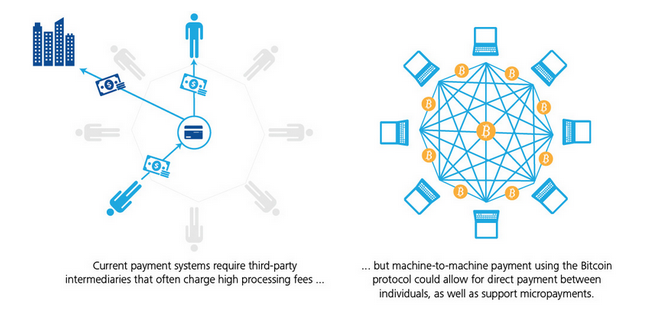
\includegraphics[scale=0.6]{Talk3/blockchain}
         \end{center}
         \caption{This is a pic FROM ILIA}
         \label{label}
       \end{figure}
   
%https://www2.deloitte.com/nl/nl/pages/innovatie/artikelen/blockchain-technology-9-benefits-and-7-challenges.html
\subsection{Benefits of Blockchain Technology}
Every technology that is centralized offers somewhere a point of failure which might be exploited by attackers and nowadays, banks are normally used by most people as a trusted middleman in order to make transaction.
Thanks to its decentralizations, blockchain will avoid the need of a trusted middleman to make transaction by connecting directly buyers and sellers.
%TODO

%http://www.huffingtonpost.com/ameer-rosic-/5-blockchain-applications_b_13279010.html
\subsection{Blockchain applications}
The most famous application of blockchain is in online trades where it gets used for transfering a cryptovalue, bitcoins.
%TODO 


%https://www.shapingtomorrow.com/home/alert/665529-Future-of--Blockchain
%http://usblogs.pwc.com/emerging-technology/the-blockchain-problem-is-a-trust-problem/
\subsection{Future of Blockchain}
%TODO 

%https://www.taylorwessing.com/download/article-how-secure-is-block-chain.html
\subsection{Blockchain security}
%TODO 


\section{Smart Contract: Introduction}
\subsection{Smart Contract: a self-executing contractual agreements}
%definition founded here: https://www.youtube.com/watch?v=FkeLDPZ-v8g&t=134s
A Smart Contract is a piece of software that stores rules for negotiating the terms of a contract, automatically verifies the contract and then executes the agreed terms. 

%https://bitsonblocks.net/2016/02/01/a-gentle-introduction-to-smart-contracts/%
\subsubsection{Traditional vs. Smart Contract}

\subsection{Ethereum: a public blockchain-based platform}
Smart contract applications based on public blockchains.


\subsubsection{Solidity: a typed JavaScript-like language}


\section{Smart Contract attacks}

\subsection{DAO: First Attack}
\subsubsection{Attack description}
\subsubsection{Exploited vulnerability}
\subsubsection{Possible solution}

\subsection{DAO: Second Attack}
\subsubsection{Attack description}
\subsubsection{Exploited vulnerability}
\subsubsection{Possible solution}

\subsection{King of The Ether Throne Attack}
\subsubsection{Attack description}
\subsubsection{Exploited vulnerability}
\subsubsection{Possible solution}

\subsection{MultiPlayer Attack}
\subsubsection{Attack description}
\subsubsection{Exploited vulnerability}
\subsubsection{Possible solution}

\subsection{Rubixi Attack}
\subsubsection{Attack description}
\subsubsection{Exploited vulnerability}
\subsubsection{Possible solution}

\subsection{Govern-Mental: First Attack}
Blablabla said asfbzasfubasbusauhfhu \cite{WinNT}.
\subsubsection{Attack description}
\subsubsection{Exploited vulnerability}
\subsubsection{Possible solution}

\subsection{Govern-Mental: Second Attack}
\subsubsection{Attack description}
\subsubsection{Exploited vulnerability}
\subsubsection{Possible solution}

%http://usblogs.pwc.com/emerging-technology/tag/blockchain/
%http://www.coindesk.com/blockchain-smart-contracts-looming-challenges/
\section{Security Challenges in Smart Contract}
\subsection{No guarantee of transaction execution}
\subsection{Slowness of Smart Contract}
\subsection{Code is slow}

\begin{thebibliography}{99}
\bibitem{ethereum1}\emph{Ethereum Homestead Release.} \url{https://www.ethereum.org} (last accessed March 2017)
\bibitem{wikipedia1}\emph{Blockchain} Wikipedia: \url{https://en.wikipedia.org/wiki/Blockchain} (last accessed February 2017)
\bibitem{blockchain1}\emph{Know More About Blockchain.} \url{https://letstalkpayments.com/an-overview-of-blockchain-technology/} (last accessed March 2017)
\bibitem{blockchain2}\emph{Blockchain Use Cases Part II.} \url{https://letstalkpayments.com/blockchain-use-cases-part-ii-non-financial-and-financial-use-cases/} (last accessed March 2017)


\bibitem{paper1}Loi Luu, Duc-Hiep Chu, Hrishi Olickel, Prateek Saxena, Aquinas Hobor: \emph{Making Smart Contracts Smarter.}. October 2016. \url{http://delivery.acm.org/10.1145/2980000/2978309/p254-luu.pdf?ip=195.176.96.218&id=2978309&acc=ACTIVE\%20SERVICE&key=FC66C24E42F07228\%2EA04051DB0C098788\%2E4D4702B0C3E38B35\%2E4D4702B0C3E38B35&CFID=926344688&CFTOKEN=88107312&__acm__=1492712435_d0f0d96ea04f8cf077c9b90253210778} (last accessed February 2016)

\bibitem{paper1}Atzei, Nicola and Bartoletti, Massimo and Cimoli, Tiziana: \emph{A survey of attacks on Ethereum smart contracts.} 2016. Cryptology ePrint Archive: Report 2016/1007, https://eprint. iacr. org/2016/1007 \url{https://eprint.iacr.org/2016/1007.pdf} (last accessed February 2017)

\bibitem{blockchain3}Investopedia: \emph{What is a Blockchain.} \url{http://www.investopedia.com/terms/b/blockchain.asp} (last accessed March 2017)

\bibitem{blockchain4}\emph{Blockchain technology: 9 benefits and 7 challenges.} \url{https://www2.deloitte.com/nl/nl/pages/innovatie/artikelen/blockchain-technology-9-benefits-and-7-challenges.html} (last accessed March 2017)

\bibitem{blockchain5}Hasse, von Perfall, Hillebrand, Smole, Lay, Charlet: \emph{Blockchain - an opportunity for energy producers and consumers?.}\url{http://www.pwc.ch/en/2017/pdf/pwc_blockchain_opportunity_for_energy_producers_and_consumers_en.pdf} (last accessed March 2017)

\bibitem{blockchain6}\emph{What is Blockchain Technology?.} \url{https://blockgeeks.com/guides/what-is-blockchain-technology/} (last accessed March 2017)
\bibitem{blockchain7}\emph{Know More About Blockchain.} \url{https://letstalkpayments.com/an-overview-of-blockchain-technology/} (last accessed April 2017)
\bibitem{blockchain8}\emph{Five Blockchain Applications That Are Shaping Your Future.}\url{http://www.huffingtonpost.com/ameer-rosic-/5-blockchain-applications_b_13279010.html} (last accessed March 2017)
\bibitem{blockchain9}\emph{Future of Blockchain.} \url{https://www.shapingtomorrow.com/home/alert/665529-Future-of--Blockchain} (last accessed February 2017)
\bibitem{blockchain10}\emph{The blockchain problem is a trust problem.}\url{http://usblogs.pwc.com/emerging-technology/the-blockchain-problem-is-a-trust-problem/} (last accessed February 2017)
\bibitem{blockchain11}\emph{How secure is blockchain?.} \url{https://www.taylorwessing.com/download/article-how-secure-is-block-chain.html} (last accessed March 2017)
\bibitem{SC1}\emph{Simple introduction to smart contracts on a blockchain.} \url{https://www.youtube.com/watch?v=FkeLDPZ-v8g&t=134s} (last accessed March 2017)
\bibitem{SC2}\emph{A gentle introduction to smart contracts.} \url{https://bitsonblocks.net/2016/02/01/a-gentle-introduction-to-smart-contracts/} (last accessed February 2017)
\bibitem{SC3}\emph{Blockchain Pros Debate Looming Challenges for Smart Contracts.} \url{http://www.coindesk.com/blockchain-smart-contracts-looming-challenges/} (last accessed April 2017)



\bibitem{blockchain0}Morabito: \emph{Blockchain Value System.} 2017. \url{http://www.springer.com/cda/content/document/cda_downloaddocument/9783319484778-c2.pdf?SGWID=0-0-45-1599947-p180347565} (last accessed March 2017)
\bibitem{SC5}\emph{title.}\url{url} (last accessed April 2017)
\bibitem{SC6}\emph{title.}\url{url} (last accessed April 2017)
\bibitem{SC7}\emph{title.}\url{url} (last accessed April 2017)
\bibitem{SC8}\emph{title.}\url{url} (last accessed April 2017)
\bibitem{SC9}\emph{title.}\url{url} (last accessed April 2017)
\bibitem{SC10}\emph{title.}\url{url} (last accessed April 2017)
\bibitem{SC11}\emph{title.}\url{url} (last accessed April 2017)
\bibitem{SC12}\emph{title.}\url{url} (last accessed April 2017)
\bibitem{SC13}\emph{title.}\url{url} (last accessed April 2017)









\end{thebibliography}
